
\chapter{Introduction}
\label{chap:intro}
In many situations, people will have to make decisions about the products they are going to purchase and how they are going to spend their money 
Traditionally, people have used a variety of strategies to solve this decision making problem: conversations with friends, obtaining information from a trusted third party, hiring an expert team or simply follow the crowd. 
%It would be great to have an affordable personal advisor who helps us make good decisions efficiently.
In the present age where e-commerce is flourishing, most e-commerce sites have very large number of products (often in millions) in their databases.
For a user wanting to purchase a product, examining all the products (eg: mobile applications) present in the catalog one after another in the hope of finding a product that is of interest to him is impractical.
Keyword search is not going to be greatly helpful because an average user does not have a clear understanding of the product space and is often unclear with what kind of products he exactly wants.

We would like to have systems that assist the user to find products of his interest and enable him to efficiently navigate through the complex product space.
\textit{Recommender systems} are constructed for this purpose - assisting a user in his/her (online) decision-making.
%In the present age when e-commerce is flourishing, sizes of product catalogs often is in thousands.
Recommender systems play an extremely important role in matching users to products or items that they might find interesting. 
They filter out huge amounts of information to give personalized suggestions that its users might be interested in. 
This reduces the cognitive effort on the users who are spared of the need to examine a large number of irrelevant items before reaching their desired product.

Recommender Systems are broadly classified into three categories: Collaborative, Content Based and Knowledge Based.

\section{Collaborative Recommender Systems}
\label{sec:CF}
 The main idea in these systems is that if users have shared the same interests in the past - if they bought or similarly rated the same items - they will also have similar tastes in the future. 
This technique is also called as \textit{Collaborative Filtering}(CF). 
Pure CF based approaches require only rating data and do not require the additional knowledge about underlying users/items. 
Hence, the algorithms are usually domain independent. Most commercial recommender systems use collaborative filtering for recommending items.
There are two main approaches to perform CF: Memory Based Approaches and Model Based Approaches

\subsection {Memory Based Approaches}
In this approach, the original rating matrix is held in memory and directly used to generate predicted ratings and recommendations. There are two popular memory based approaches:\\
\textbf{User based Nearest Neighbor(NN) Recommendation:} Given a user \textit{u}, the system computes top \textit{K} similar users to \textit{u} according to a pre-defined similarity measure. It recommends the items that haven't been rated/purchased by \textit{u} but liked by the top \textit{K} similar users.\\
\textbf{Item based NN Recommendation:} Given a user \textit{u}, the system recommends items that have received similar ratings to the ones that \textit{u} had previously liked.
 


\subsection {Model Based Approaches}
As opposed to memory based approaches that use the ratings matrix to directly generate predictions, model based approaches learn models corresponding to each item and each user from the ratings matrix. The learned models are used to make predictions at run time.
Model based approaches perform well in practice for large datasets.
\textit{Matrix factorization} is a popular model based approach. The superiority of matrix factorization techniques over traditional CF in improving prediction accuracy was clearly seen during \textit{'The Netflix prize'} competition(\cite{koren}).
Broadly speaking, matrix factorization methods derive a set of latent(hidden) factors from the rating patterns and characterize each item and user as vectors of these factors.
In the movie domain, such latent factors can correspond to some aspects of a movie like genre, but most of them are completely uninterpretable (\cite{koren})


\subsection{Limitations of CF}
\label{sec:limCF}
\textbf{Cold Start Problem:} To provide recommendations for a user \textit{u}, pure CF techniques rely on \textit{u}'s ratings. This means that for a new user who has not yet rated a single item, there is no way of generating personalized recommendations (\textit{new-user problem}). 
Similarly, for a new item that has been recently added to the catalog and has not been rated by a single user, there is no way for it to be recommended to a user (\textit{new-item problem}).\\
\textbf{Sparsity:} The relevance and accuracy of CF recommender's predictions is high when the user-item ratings matrix is dense.
But in real-world systems, the rating matrices are typically very sparse and thus, the quality of recommendations of pure CF approaches may not be good.
As an example, consider a user \textit{u} whose rating pattern is very different from most of the other users. 
He would find it difficult to receive useful recommendations because the number of similar users to \textit{u} is very less(\cite{balab1997}).




%

%

\section{Content Based Recommender Systems}
\label{sec:content}
Collaborative Filtering Systems do not require any knowledge about underlying users/items to make recommendations.
As opposed to this, content based recommender systems rely on item descriptions and explicit/learned user profiles to recommend items.
For example, if the recommender system knows that \textit{Harry Potter} is a fantasy novel and the user Alice has always like fantasy novels, the system can recommend the new \textit{Harry Potter} book right away. 
Content-based recommender systems need not rely on the existence of a large user base to generate recommendations.
It overcomes the cold-start problem described in Section ~\ref{sec:limCF}. However, item characteristics are hard to acquire normally and hence, they have to be entered manually into the system, which can be potentially expensive for some domains (Eg: music).

Having its roots in \textit{Information Retrieval}(IR), content based recommendation most often focuses on textual products - items which can be described in terms of textual features (Eg: documents, news articles and web sites).
Most news recommendation systems use content based recommendation to recommend relevant news articles to the users.
A news recommendation system typically recommends news articles by comparing the main keywords of a news article with the keywords in articles that the user has rated highly in the past.
There are two ways in which content based systems can create user-profiles- 
by explicitly asking the user to rate a set of items/topics/categories when the user is new to the system
or by "learning" the user profile automatically by examining the user's past behavior/ratings.
Learning user profiles from user's past behavior can be expensive and sometimes not be accurate because of time-effects(user's interests changing over time) and sparsity of user ratings.
But it has the advantage that it requires no effort from the user.

\subsection{Limitations of Content-based Recommendation}
\textbf{Limited Content Analysis:} Content-based recommender systems perform a shallow content analysis which might not be sufficient in many scenarios. Particularly, for recommending resources such as web pages, aspects other than the keywords like aesthetics, usability and correctness of hyperlinks play a part in establishing the quality of recommendations (\cite{jannach}).
Also, content based recommender systems using limited content analysis based on just keywords, have no way to distinguish between well written and poorly written articles, both of which use the same set of keywords. 
Also, feature extraction techniques for text documents is relatively mature, but the same cannot be said about many multimedia objects like images and videos.
Hence, the usability of content-based recommender systems is limited in multimedia domain. (\cite{adom2005})\\
\\
\textbf{Over-specialization:}  Another drawback of content based recommender systems is that they often tend to recommend items that the user might have already seen/rated. 
A general goal therefore is to increase the serendipity of the recommendation lists - that is, to include "unexpected" items in which the user might be interested in.
The system described by \cite{billsus} therefore defines a threshold to filter out not only items that are too different from the user profile but also those that are too similar.\\
\\
\textbf{New user problem:} The new user problem discussed in Section \ref{sec:limCF} also exists for content based recommender systems.
Although content-based techniques do not require a large user community, they require at least an initial set of ratings from the user, typically a set of explicit \textit{like} and \textit{dislike} statements.
Content-based recommenders do not have the new item problem. 
Given a new item, the recommender system matches the new item's features to existing user profiles and recommends it directly to relevant users.

\section{Knowledge Based Recommender Systems}
Collaborative filtering systems, discussed in Section \ref{sec:CF} suggest items to user based on user's past ratings.
Content based recommender systems, discussed in Section \ref{sec:content} recommend items whose features match the user's profile.
Consider some high-risk product domains like houses, cars, computers etc.
Typically, users do not buy a house, a car or a computer very frequently. 
In such a scenario, both collaborative-filtering or content-based recommender systems may not be able to generate relevant recommendations because of the low number of available ratings.
User-profiles learnt by content-based systems may not be useful for making recommendations due to a heavy influence of time effects(change in user's interests and product catalogs with time). 
For example, if a user has given a high rating to a 'Pentium III' computer four years ago, the recommender system cannot rely on that rating for generating relevant recommendations for the current day.
In complex and high-risk product domains such as computers, customers often want to define their requirements explicitly - for example, "the maximum price of the computer should be \$1400 and the hard-disk capacity should be at least 500GB".
Knowledge based systems are used to provide recommendations in such scenarios.
%In knowledge based systems, recommendations are made taking into account the explicit user preferences and the rich knowledge base available.

Knowledge-based recommender systems can be divided into two categories: constraint-based and case-based.
Constraint-based recommender systems rely on explicit recommendation rules and case-based recommender systems use similarity/utility measures to generate recommendations. 
A case-based recommendation is typically generated based on similarity of the items in the case base with the user defined query.
Case-based recommendation and the algorithm for MAUT based recommendation are discussed in detail in Chapter \ref{chap:background}.

Recommendation process of knowledge-based recommender applications is highly interactive, a foundational property that is a reason for their characterization as \textit{\textbf{conversational systems}}. The recommender system that we consider in this project is a conversational recommender system.
Conversational systems assume that a user's initial query is merely a starting point for search, perhaps even an unreliable starting point. The job of a conversational system is to help the user refine his initial preference query as the interactions proceed.
\subsection{Critiquing}
\label{sec:critiquing}

\begin{figure}
\centering
\begin{minipage}{.5\textwidth}
  \centering
  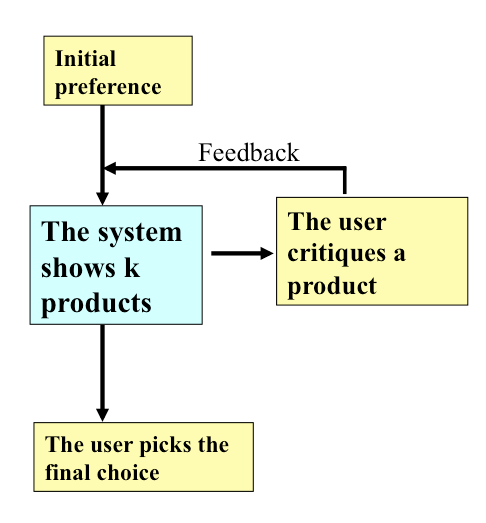
\includegraphics[width=1\linewidth]{figures-bharath/critiquing.png}
  \captionof{figure}{Critiquing}
  \label{fig:critiquing}
\end{minipage}%
\begin{minipage}{.5\textwidth}
  \centering
  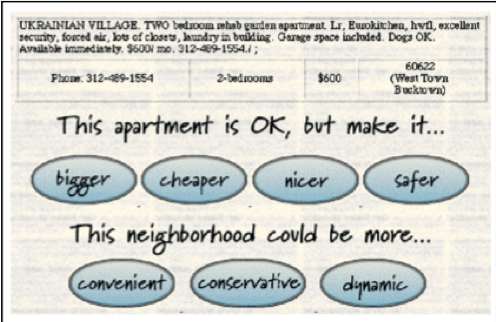
\includegraphics[width=1\linewidth]{figures-bharath/rentMe.png}
  \captionof{figure}{RentMe Recommender System: \cite{burkeRentMe}}
  \label{fig:rentMe}
\end{minipage}
\end{figure}
\textit{\textbf{Critiquing}} is one of the most popular forms of feedback in conversational recommender systems. In each interaction cycle, the user is presented with a list of products.
User selects a product and expresses directional preference(s) over one or more item feature values. 
For example, one might indicate that he is looking for a less expensive restaurant or a more formal setting(Figure \ref{fig:rentMe}). These are two individual critiques, first critique being on the \textit{price} attribute and the second critique on the \textit{setting} attribute. 
The recommender updates it's user model according to this feedback and provides another set of products and proceeds to the next recommendation cycle. This continues till the user finally chooses a product. (Figure \ref{fig:critiquing})

\textit{\textbf{Unit critiques}} allow users to express their preference over one attribute in each interaction cycle. \textit{\textbf{Compound critiques}} enable users to input their preferences on several attributes at a time. This can potentially shorten the number of interaction cycles in finding a target product.
The early FindMe Systems \cite{burkeEarlierSystems} had \textit{\textbf{static critiques}}. The critiques wouldn't change when users selected a particular critique. 
This can lead to some serious limitations.
For example, the critique 'cheaper' would continue to be visible, even if there are no cheaper apartments available and when user clicks on 'cheaper', there would be no results displayed at all.
Static critiques also do not represent the best set of tweaks that a user will want to make given his preference model.
The notion of \textit{\textbf{dynamic critiquing}} was first proposed by \cite{mccarthy2004dynamic} to overcome the limitations of static critiques.
Compound critiques are generated on-the-fly for each recommendation cycle. Dynamic critiquing has been shown to improve user-experience and lower the average number of interaction cycles it takes for a customer to find his desired product.

There are two popular approaches to dynamic critiquing: Apriori algorithm based generation of compound critiques (\cite{mccarthy2004dynamic}) and MAUT based generation of compound critiques (\cite{mautPaper}). 
The algorithm for MAUT based recommendation is discussed in Section \ref{sec:maut}.

\subsection{Limitations of Knowledge based recommendation}
One of the obvious limitations of knowledge based recommenders is that they require a high level of knowledge engineering effort.
One needs to define local similarity functions, utility measures, assign weights to features etc. and the recommendation efficiency and accuracy is very sensitive to how we define them.
%Offline evaluation is generally not very reliable in these systems.
%We need to conduct live user studies to prove the efficiency of 

\section{Our contribution: Improvements to MAUT based recommendation}
MAUT based recommendation has been shown using both offline experiments and live user studies (Sections \ref{sec:offline} and \ref{sec:liveUser}) to be one of the best performing recommendation algorithms in the domain of critiquing based recommendation.
Our goal in this project is to improve the performance of MAUT based recommendation.
To this end, we have proposed several algorithms in Chapter \ref{chap:modifications} that led to significant performance improvements.

\section{Organization of the Thesis}
In Chapter \ref{chap:background}, we present an overview of case based recommendation and discuss the algorithms for Apriori and  MAUT based generation of dynamic critiques in detail. We also discuss the offline experiments and live user studies that were conducted in the past to compare the performances of Apriori and MAUT based critiquing.
In Chapter \ref{chap:modifications}, we describe several modifications proposed to MAUT based recommendation algorithm that have led to significant performance improvements.
In Chapter \ref{chap:results}, we describe the experimental procedure and report the the improvements achieved by each of the proposed modifications.
Finally, we present conclusions and possible directions for future work in Chapter \ref{chap:conclusions}.
